\section{Increment-Schedule Sensitivity of the Chaboche-v1 UMAT}

This section freezes the Stage 3 sensitivity study that compared three controlled DMAX settings for the same 20-cycle Chaboche-v1 simulation.

The question is whether accumulated viscoplastic strain remains invariant under time-increment refinement. It does not. The cycle-20 accumulated strain increases monotonically as DMAX decreases, so the UMAT remains increment-size sensitive and Level-3 STATEV injection stays deferred.

\subsection{Cycle-20 Summary}

\begin{table}[htbp]
\centering
\small
\begin{tabular}{lrrrrr}
\toprule
\textbf{Case} & \textbf{DMAX} & \textbf{INC limit} & \textbf{STATEV1 @ cycle 20} & \textbf{Rel. diff. vs ref.} & \textbf{Avg $S_{11}$ @ cycle 20} \\
\midrule
Original-output baseline & 0.020 & 4000 & 0.142025694251 & 0\% & 376.434143066 \\
DMAX-refined case & 0.010 & 4000 & 0.143569096923 & 1.0867\% & 380.566436768 \\
Fine DMAX case & 0.005 & 6000 & 0.145257070661 & 2.2752\% & 385.053924561 \\
\bottomrule
\end{tabular}
\caption{Stage 3 increment-schedule sensitivity summary for the Chaboche-v1 UMAT. The reference value for STATEV1 at cycle 20 is 0.142025694251.}
\label{tab:stage3_increment_sensitivity}
\end{table}

\subsection{STATEV1 Versus DMAX}

The first sensitivity plot shows the final cycle-20 accumulated viscoplastic strain against the maximum allowed increment size. The trend is monotonic: smaller DMAX produces larger accumulated \texttt{STATEV1}.

\begin{figure}[htbp]
    \centering
    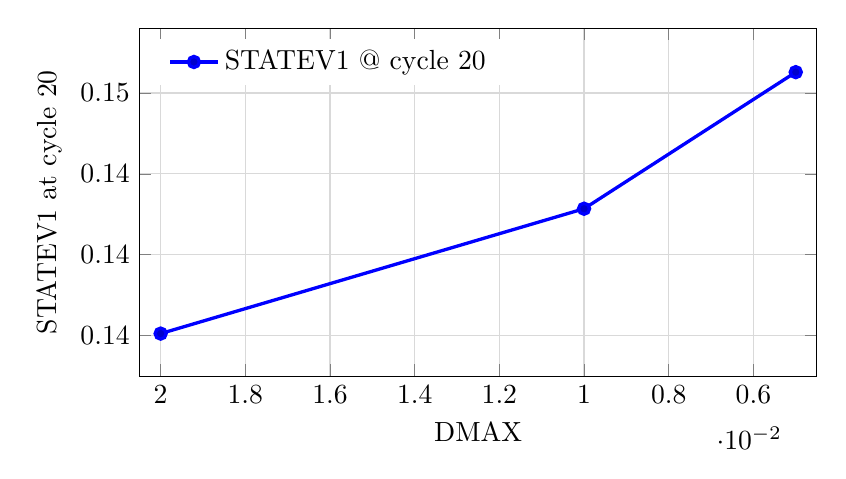
\begin{tikzpicture}
    \begin{axis}[
        width=0.84\textwidth,
        height=6cm,
        xlabel={DMAX},
        ylabel={STATEV1 at cycle 20},
        x dir=reverse,
        grid=both,
        grid style={gray!20},
        major grid style={gray!30},
        legend style={draw=none, at={(0.03,0.97)}, anchor=north west},
        ymin=0.1415,
        ymax=0.1458,
        xmin=0.0045,
        xmax=0.0205,
    ]
    \addplot+[mark=*, very thick, blue] coordinates {
        (0.020,0.142025694251)
        (0.010,0.143569096923)
        (0.005,0.145257070661)
    };
    \addlegendentry{STATEV1 @ cycle 20}
    \end{axis}
    \end{tikzpicture}
    \caption{Cycle-20 STATEV1 versus DMAX for the three completed Stage 3 runs.}
    \label{fig:stage3_statev1_vs_dmax}
\end{figure}

\subsection{STATEV1 Evolution Across Cycles}

The second plot shows the cycle-end evolution of STATEV1 for the three completed cases. It confirms that the cases separate progressively as the increment schedule becomes finer. The source SVG versions of the Stage 3 plots are archived in the thesis package figures folder alongside this LaTeX-generated version of the same result.

\pgfplotstableread[col sep=comma]{tables/chaboche_eps005_20cycles_dt_original_output_statev_history.csv}\stageThreeOriginal
\pgfplotstableread[col sep=comma]{tables/chaboche_eps005_20cycles_dtmax_0p01_statev_history.csv}\stageThreeRefined
\pgfplotstableread[col sep=comma]{tables/chaboche_eps005_20cycles_dtmax_0p005_inc6000_statev_history.csv}\stageThreeFine

\begin{figure}[htbp]
    \centering
    \begin{tikzpicture}
    \begin{axis}[
        width=0.84\textwidth,
        height=7cm,
        xlabel={Cycle},
        ylabel={STATEV1},
        grid=both,
        grid style={gray!20},
        major grid style={gray!30},
        legend style={draw=none, at={(0.03,0.97)}, anchor=north west},
        xmin=1,
        xmax=20,
        ymin=0,
    ]
    \addplot+[blue, very thick, mark=*, mark size=1.5pt] table[x=cycle,y=STATEV1_end] {\stageThreeOriginal};
    \addplot+[red, very thick, mark=square*, mark size=1.5pt] table[x=cycle,y=STATEV1_end] {\stageThreeRefined};
    \addplot+[green!60!black, very thick, mark=triangle*, mark size=1.5pt] table[x=cycle,y=STATEV1_end] {\stageThreeFine};
    \addlegendentry{DMAX = 0.020}
    \addlegendentry{DMAX = 0.010}
    \addlegendentry{DMAX = 0.005}
    \end{axis}
    \end{tikzpicture}
    \caption{Cycle-end STATEV1 evolution for the three completed increment-schedule cases.}
    \label{fig:stage3_statev1_vs_cycle}
\end{figure}

\subsection{Interpretation}

The Chaboche-v1 UMAT shows a monotonic increase in accumulated viscoplastic strain as DMAX decreases, confirming increment-size sensitivity. The DMAX = 0.005 run required a larger increment limit because the earlier INC = 2500 deck failed with too many increments; the corrected INC = 6000 run completed successfully and became the final Stage 3 data point. The practical implication is unchanged: Level-3 STATEV injection and a full Nesnas--Saanouni restart-level cycle jump remain deferred until UMAT integration robustness is improved.